\chapter{Migrar tu estación a la librería}\label{cap:migracion}

Este es el capítulo para el que se ha hecho todo lo demás. Cuenta, paso a paso, cómo llevar tu estación a \lib\ \textbf{sea cual sea el punto en el que estés}: si no has empezado, si lo tienes todo mezclado en un bloque enorme, o si ya tienes una estructura parecida a la de la práctica.

\begin{idea}
La migración no consiste en \emph{reescribir} tu estación, sino en \textbf{separarla en dos}: lo común (que ahora lo hace la librería, y que tú borras) y lo propio (tu aplicación, que conservas y adaptas). Casi todo el trabajo es decidir qué parte de tu código es cuál.
\end{idea}

\section{Antes de empezar}

\subsection{Las cinco fases}
\begin{figure}[ht]
\centering
\begin{tikzpicture}[x=1cm,y=1cm]
\newcommand{\fase}[5]{\node[#2,minimum width=2.45cm,minimum height=1.9cm,font=\sffamily\footnotesize,text width=2.2cm,align=center] (f#1) at (#1*2.9-5.8,0) {\textbf{#1}\\[-1pt]\textbf{#3}\\[1pt]{\scriptsize #4}};}
\fase{1}{caja}{Preparar}{copia de seguridad, inventario, hardware}{}
\fase{2}{libcaja}{Instalar}{la librería y los tags (cap.\ \ref{cap:instalacion})}{}
\fase{3}{caja}{Separar}{qué se va y qué se queda de tu código}{}
\fase{4}{appcaja}{Reconstruir}{tu aplicación con el contrato}{}
\fase{5}{caja}{Conectar y probar}{\cod{Main} y pruebas}{}
\foreach \i/\j in {1/2,2/3,3/4,4/5} \draw[flecha] (f\i.east) -- (f\j.west);
\end{tikzpicture}
\caption{Las cinco fases de la migración. Entre una y otra se compila: no sigas si hay errores.}
\end{figure}

\subsection{Cuánto tiempo lleva}
Con el código que ya tienes, calcula entre dos y cuatro horas la primera vez: una para preparar e instalar, una a dos para separar y reconstruir, y una para probar. La primera estación de cada uno es la lenta; el resto de la gente va más deprisa porque ya ha visto el patrón.

\subsection{Cuatro normas}
\begin{enumerate}[leftmargin=1.2cm,label=\textbf{N\arabic*.}]
\item \textbf{Copia de seguridad antes de tocar nada.} Archiva tu proyecto (\menu{Project $\rightarrow$ Archive}) con la fecha en el nombre.
\item \textbf{No borres tu código antiguo: apártalo.} Crea una carpeta \menu{Antiguo} dentro de \menu{Program blocks} y mueve ahí lo que sustituyas. Hasta que todo funcione, es tu red de seguridad.
\item \textbf{Un paso cada vez y compilando.} Así sabes siempre qué cambio ha roto algo.
\item \textbf{No edites los bloques de la librería.} Si algo no te encaja, mira el capítulo~\ref{cap:problemas} o pide un cambio (capítulo~\ref{cap:mantenimiento}).
\end{enumerate}

\section{¿En qué punto estás?}\label{sec:punto}
Elige la fila que más se parezca a tu situación. Cada una te manda al camino que debes seguir.

\begin{center}
\small
\begin{tabularx}{\textwidth}{>{\bfseries}p{4.1cm}Xp{2.0cm}}
\toprule
Tu situación & Qué hacer & Camino \\
\midrule
Solo tienes el hardware configurado, o muy poco programado & Empieza con la plantilla. Es lo más fácil. & A (sección~\ref{sec:camino-a}) \\
Tienes la estructura de la práctica: bloques separados de modos, cinta, RFID y aplicación & Sustituye los tres primeros por la librería; conserva y adapta tu aplicación. & B (sección~\ref{sec:camino-b}) \\
Tienes todo en uno o dos bloques, mezclado & Primero hay que separar (sección~\ref{sec:separar}), y luego sigues el camino B. & B, con separación \\
Tu código ya lee o escribe el tag RFID a su manera (una palabra, otra dirección, otro formato) & Sigue el camino que te toque y haz además la sección~\ref{sec:rfid-propio}. & A o B, más \S\,\ref{sec:rfid-propio} \\
Tu estación tiene hardware especial (cámara PROFINET, PLC Festo…) & Sigue igual: ese hardware es parte de tu aplicación, la librería no lo toca. & A o B \\
\bottomrule
\end{tabularx}
\end{center}

\begin{figure}[ht]
\centering
\begin{tikzpicture}[x=1cm,y=1cm]
\node[caja,fill=white] (q1) at (0,0) {¿Tu proyecto ya tiene programados\\los botones, la cinta y el RFID?};
\node[libcaja] (A) at (-6.0,0) {\textbf{Camino A}\\proyecto nuevo\\con la plantilla};
\node[caja,fill=white] (q2) at (0,-2.4) {¿Tu aplicación está en un bloque\\propio, separada de lo anterior?};
\node[libcaja] (B) at (6.0,-2.4) {\textbf{Camino B}\\sustituir lo común,\\adaptar tu aplicación};
\node[appcaja] (S) at (0,-4.9) {\textbf{Camino B con separación}\\(antes, separar tu código en\\«lo común» y «lo propio»)};
\draw[flecha] (q1.west) -- node[etiqueta,above] {no} (A.east);
\draw[flecha] (q1.south) -- node[etiqueta,right] {sí} (q2.north);
\draw[flecha] (q2.east) -- node[etiqueta,above] {sí} (B.west);
\draw[flecha] (q2.south) -- node[etiqueta,right] {no, está todo mezclado} (S.north);
\draw[flecha] (S.east) -| (B.south);
\end{tikzpicture}
\caption{Cómo elegir el camino.}
\end{figure}

\section{Camino A: empezar con la plantilla}\label{sec:camino-a}
Es el camino corto: tu proyecto casi no tiene lógica, así que se construye todo sobre la librería desde el principio. Calcula una hora u hora y media.

\reiniciapaso
\paso{Prepara el proyecto}
Crea un proyecto con tu CPU y configura el hardware de la estación: las dos tarjetas de entradas, las dos de salidas y el maestro IO-Link con el lector y el stopper. Las direcciones tienen que ser las de la tabla de la sección~\ref{sec:tags}. Si ya tienes un proyecto con el hardware hecho (por ejemplo, el de la práctica), úsalo y borra lo demás.

\paso{Instala la librería}
Capítulo~\ref{cap:instalacion}: desarchivar, arrastrar \cod{Est\_FB\_Estacion} y copiar de la plantilla los tags, \cod{DB\_Estacion}, \cod{Est\_FB\_App\_Plantilla} y \cod{Main}.

\paso{Crea tus señales físicas}
Haz el inventario (lista~1 de la sección~\ref{sec:fase1}) y crea los tags de tus sensores y actuadores, con un UDT propio o sueltos.

\paso{Convierte la plantilla en tu aplicación}
Copia \cod{Est\_FB\_App\_Plantilla}, renómbrala \cod{FB\_App\_}\emph{tu estación} y sigue los seis pasos de la fase~4 (sección~\ref{sec:fase4}): tus señales, tus bytes del tag, tu condición de reposo y tu secuencia.

\paso{Conecta y calcula tus máscaras}
En \cod{Main}, cambia la llamada de la plantilla por tu aplicación y pon tus máscaras (capítulo~\ref{cap:mapa}). Si tu aplicación tiene señales físicas, cablea esos pines a tus tags (sección~\ref{sec:fase5}).

\paso{Compila y prueba}
Compila y haz las pruebas del capítulo~\ref{cap:pruebas}, empezando por la escritura desactivada.

\comprobar{Compila con 0 errores y las 12 pruebas de aceptación pasan.}

\section{Camino B: migrar un proyecto existente}\label{sec:camino-b}
Es el camino largo, pero se hace en cinco fases que conviene hacer \textbf{en este orden}. Cada fase termina con una comprobación: si no la cumples, no sigas.

\section{Fase 1: preparar}\label{sec:fase1}
\reiniciapaso
\paso{Haz la copia de seguridad}
\menu{Project $\rightarrow$ Archive}, tipo \menu{Compressed TIA Portal project archive}, con un nombre como \texttt{MiEstacion\_antes\_de\_CPLabCore.zap20}.

\paso{Rellena el inventario de tu estación}
Es una hoja con cuatro listas (la versión imprimible está en el apéndice~\ref{ap:checklists}). Es lo más útil de toda la migración, porque te obliga a decidir qué es tuyo y qué es común:

\begin{center}
\small
\begin{tabularx}{\textwidth}{>{\bfseries}p{4.2cm}X}
\toprule
Lista & Qué apuntar \\
\midrule
1. Mis señales físicas & Todos los sensores y actuadores que \textbf{no} son botonera, cinta, stopper ni RFID. Con su dirección actual. (Esas son tu aplicación.) \\
2. Mis datos del palet & Qué información lees del tag y cuál escribes. Con su byte según el Excel del grupo (capítulo~\ref{cap:mapa}). \\
3. Cuándo puedo empezar & La condición que tiene que cumplir tu mecanismo para estar en reposo y recibir un palet. \\
4. Cuándo he terminado & La condición con la que sabes que has acabado con el palet. \\
\bottomrule
\end{tabularx}
\end{center}

\paso{Comprueba tu hardware}
Abre \menu{Device configuration} y comprueba que tus módulos tienen las direcciones de la tabla de la sección~\ref{sec:tags}: entradas digitales en 0 y 1, salidas digitales en 0 y 1, y el maestro IO-Link con el lector en 10 y el stopper en 42. Son las mismas en todas las estaciones de la CP-Lab. Si alguna es distinta, apúntala: en la fase 2 la corregirás en el tag, no en la librería.

\comprobar{Tienes la copia, el inventario relleno y la lista de direcciones que no coinciden (si hay alguna).}

\section{Fase 2: instalar}
Sigue el capítulo~\ref{cap:instalacion}: desarchivar la librería, arrastrar \cod{Est\_FB\_Estacion} (con sus dependencias) y copiar los tags y los bloques de la plantilla. Algunas notas especiales para un proyecto que ya tiene cosas:

\begin{itemize}
\item \textbf{Tags que ya tengas con las mismas direcciones.} Si en tu tabla de variables hay tags sueltos para los botones, la cinta o el RFID (por ejemplo, \cod{Boton\_marcha} en \cod{\%I1.0}), son los que sustituyen los siete tags de la librería. Muévelos a otra tabla (\menu{Antiguo}) o desactívalos; no los borres de momento, porque tu código antiguo los usa. La librería usa tags \emph{con estructura} en esas direcciones.
\item \textbf{Tu aplicación sigue con sus propios tags} y UDT: no les afecta nada de esto.
\item \textbf{Bloques con los mismos nombres.} Si ya tienes un \cod{Main} o un \cod{FB1}, TIA te preguntará qué hacer al copiar. En el \cod{Main}, no sobrescribas todavía.
\end{itemize}

\comprobar{El software compila y no hay errores en los bloques de la librería. Los errores que queden son de tu código antiguo (que usa nombres que ya no existen) y se resuelven en la fase 3.}

\section{Fase 3: separar tu código}\label{sec:separar}
Es el momento de decidir, línea a línea, qué se queda y qué se va. La regla es sencilla:

\begin{idea}
\textbf{Si el código tiene que ver con los botones, la cinta, el stopper, el lector RFID o la secuencia «leer, trabajar, escribir», ya lo hace la librería: sobra. Si mueve tu mecanismo o inspecciona, pone o procesa una pieza, es tu aplicación: se queda.}
\end{idea}

La tabla de la página siguiente traduce las cosas más habituales. Mira cada parte de tu código y búscala en la columna izquierda.

\begin{center}
\small
\begin{longtable}{>{\raggedright\arraybackslash}p{5.6cm}>{\raggedright\arraybackslash}p{2.0cm}>{\raggedright\arraybackslash}p{6.2cm}}
\toprule
\textbf{Si tu código hace\dots} & \textbf{Qué hacer} & \textbf{Ahora lo hace\dots} \\
\midrule\endhead
Leer el botón de marcha, paro o rearme, el selector manual/auto o la seta & \textcolor{rojo}{Borrar} & \cod{Est\_FB\_Modo}. Entradas en \cod{Entradas\_Basico}. \\
Decidir si hay emergencia y cómo se sale de ella & \textcolor{rojo}{Borrar} & \cod{Est\_FB\_Modo}. Tu aplicación recibe \cod{Emergencia}. \\
Encender las luces de marcha, rearme, ciclo y emergencia & \textcolor{rojo}{Borrar} & \cod{Est\_FB\_Estacion}. Tú puedes pedir rearme con \cod{App\_rearme\_requerido} y alarma con \cod{App\_alarma}. \\
Mover la cinta, bajar o subir el stopper, contar palets & \textcolor{rojo}{Borrar} & \cod{Est\_FB\_Cinta}. Si tu mecanismo estorba, \cod{Inhibir\_cinta}. \\
Detectar que el palet ha llegado al tope & \textcolor{rojo}{Borrar} & \cod{Est\_FB\_Cinta}: \cod{Palet\_en\_posicion}. La aplicación empieza con \cod{App\_inicio}. \\
Dar la orden de leer el RFID, esperar el resultado, gestionar errores y tiempos & \textcolor{rojo}{Borrar} & \cod{Est\_FB\_RFID}. \\
Dar la orden de escribir el RFID y esperar el resultado & \textcolor{rojo}{Borrar} & \cod{Est\_FB\_RFID}. \\
La secuencia «llega palet, leer, trabajar, escribir, soltar» & \textcolor{rojo}{Borrar} & \cod{Est\_FB\_Estacion} (la secuencia del palet). \\
Una condición como «puedo arrancar» & \textcolor{azul}{Convertir} & \cod{App\_en\_reposo}. \\
Una señal como «he terminado» & \textcolor{azul}{Convertir} & \cod{App\_terminada} (y mantenerla hasta que \cod{App\_inicio} baje). \\
Usar datos que leíste del tag (por ejemplo, la calidad) & \textcolor{azul}{Convertir} & Leer \cod{Imagen\_palet[n]}. El byte tiene que estar en \cod{Mascara\_lectura}. \\
Guardar resultados en el tag & \textcolor{azul}{Convertir} & Escribir \cod{Imagen\_palet[n]}. El byte tiene que estar en \cod{Mascara\_escritura}. \\
Parar tus actuadores en emergencia & \textcolor{verde!60!black}{Conservar} & Dentro de tu aplicación, con la señal \cod{Emergencia}. \\
Mover tu mecanismo, activar tus sensores y actuadores, temporizar tus pasos & \textcolor{verde!60!black}{Conservar} & Dentro de tu aplicación, en el estado de «trabajo». \\
Mostrar cosas en la HMI & \textcolor{verde!60!black}{Conservar} & Tu HMI lee las variables de tu aplicación, o \cod{DB\_Estacion}. La librería no toca la HMI. \\
Contadores de piezas, estadísticas, registros & \textcolor{verde!60!black}{Conservar} & En tu aplicación o en tu propio bloque. \\
\bottomrule
\end{longtable}
\end{center}

\begin{ojo}
\textcolor{rojo}{\textbf{Borrar}} no significa eliminarlo ya: significa que \emph{sobra}. Muévelo a la carpeta \menu{Antiguo}. \textcolor{azul}{\textbf{Convertir}} significa que la idea se queda, pero ahora se expresa con una señal del contrato. \textcolor{verde!60!black}{\textbf{Conservar}} es tu aplicación.
\end{ojo}

\subsection{Si tienes todo mezclado en un solo bloque}
Es el caso más frecuente en los primeros intentos y no es un problema, solo requiere un paso más. Recomendación:

\paso{Duplica el bloque grande}
Haz una copia con otro nombre (por ejemplo, \cod{FB\_Antiguo}). Trabaja sobre la copia para tener siempre el original.

\paso{Marca con comentarios}
Recorre el código y pon al margen una etiqueta en cada tramo: \texttt{//[BORRAR]}, \texttt{//[CONVERTIR]} o \texttt{//[APP]}, según la tabla anterior.

\paso{Pasa a un bloque nuevo solo lo que sea \texttt{[APP]} o \texttt{[CONVERTIR]}}
Crea la aplicación nueva con la plantilla (fase 4) y copia ahí únicamente esos tramos. El resto no se copia.

\comprobar{Tienes dos cosas: un bloque antiguo apartado, intacto, y una lista clara (los comentarios) de qué parte pasa a la aplicación.}

\section{Fase 4: reconstruir tu aplicación}\label{sec:fase4}
Aquí se construye tu aplicación sobre la plantilla. Se hace en seis pasos.

\reiniciapaso
\paso{Copia la plantilla con tu nombre}
Copia \cod{Est\_FB\_App\_Plantilla} y renómbrala \cod{FB\_App\_}\emph{tu estación} (por ejemplo, \cod{FB\_App\_Press}). Se queda como bloque tuyo, sin vínculo con la librería.

\paso{Añade tus señales físicas a la interfaz}
En el apartado \texttt{VAR\_INPUT} añade tus sensores, y en \texttt{VAR\_OUTPUT} tus actuadores (con un tipo \texttt{Bool}, o el que necesites). Sácalos de tu inventario, lista~1. Los ejemplos del apéndice~\ref{ap:listados} lo hacen así y es la forma más sencilla: la aplicación no depende de ningún UDT y el cableado se hace en \cod{Main}.

\begin{consejo}
Si ya tienes un UDT con tus entradas y salidas (como \cod{UDT\_Entradas\_APP}), puedes dejarlo: usa \cod{Entradas\_app} y \cod{Salidas\_app} con ese tipo, y cablea los tags en \cod{Main}. Es lo que hace \cod{FB\_App\_Out}.
\end{consejo}

\paso{Declara tus bytes del tag}
En \texttt{VAR CONSTANT} escribe un \cod{IDX\_...} por cada byte que lees o escribes (inventario, lista~2), con el número de byte del Excel. Y apunta también los bits que uses, como \cod{BIT\_PRESS}. Cada byte que escribas tiene que estar en tu \cod{Mascara\_escritura}; cada byte que leas o escribas, en tu \cod{Mascara\_lectura}. Calcula las máscaras con el método de la sección~\ref{sec:calculo-mascara}.

\paso{Traslada tu condición de reposo}
En el estado 0 de la plantilla, sustituye \cod{App\_en\_reposo := TRUE} por tu condición (inventario, lista~3): por ejemplo, «prensa arriba» o «garra abierta y eje referenciado».

\paso{Traslada tu secuencia al estado de trabajo}
Pega la secuencia de tu mecanismo (lo marcado \texttt{[APP]}) dentro del estado 10 de la plantilla. Si tiene varias etapas, convierte el estado 10 en varios (10, 20, 30\dots), y cuando acabe la última, salta al estado de fin. En cada etapa donde antes leías el tag, usa \cod{Imagen\_palet[IDX\_...]}; donde lo escribías, asigna a la imagen.

\paso{Termina bien: resultado y mantén}
Antes del estado de fin, deja escritos en la imagen todos tus resultados. En el estado de fin, la plantilla ya hace lo correcto: \cod{App\_terminada} verdadera hasta que \cod{App\_inicio} baje, y vuelta a reposo. No lo cambies.

\comprobar{Tu aplicación compila sola. Ya cumple el contrato (revisa las cinco comprobaciones al final del capítulo~\ref{cap:contrato}).}

\subsection{Un ejemplo de antes y después}
Para ver el patrón, aquí va un caso inventado y simplificado de una estación de prensa programada «a la antigua», con todo mezclado, y cómo queda con la librería. No es ningún proyecto real: sirve para ver qué se va y qué se queda.

\begin{lstlisting}[caption={Antes: todo mezclado (ejemplo ilustrativo).}]
CASE #etapa OF
  0: // esperar
     IF #Boton_marcha AND NOT #Emergencia THEN #etapa := 1; END_IF;       // [BORRAR] botonera
  1: // llega palet
     #Cinta := TRUE;                                                       // [BORRAR] cinta
     IF #Sensor_tope THEN #Cinta := FALSE; #etapa := 2; END_IF;            // [BORRAR]
  2: // leer RFID
     #Tag_leer := TRUE; #Tag_direccion := 0;                               // [BORRAR] RFID
     IF #Tag_leido AND #Tag_listo THEN                                     // [BORRAR]
        #Golpes := #Tag_datos[13];                                         // [CONVERTIR] leer byte 13
        #etapa := 3;
     END_IF;
  3: // prensar
     #Prensa_bajar := TRUE;                                                // [APP]
     IF #Prensa_abajo THEN #Prensa_bajar := FALSE; #etapa := 4; END_IF;    // [APP]
  4: // escribir RFID
     #Tag_datos_a_escribir[16] := #Golpes;                                 // [CONVERTIR] escribir byte 16
     #Tag_escribir := TRUE;                                                // [BORRAR]
     IF #Tag_escrito THEN #etapa := 5; END_IF;                             // [BORRAR]
  5: // soltar palet
     #Stopper_bajar := TRUE; #Cinta := TRUE;                               // [BORRAR]
END_CASE;
\end{lstlisting}

\begin{lstlisting}[caption={Después: solo la aplicación (el patrón; el ejemplo completo está en el apéndice).}]
CASE #Etapa_app OF
  0: #App_en_reposo := #Prensa_arriba;                                    // tu condicion de reposo
     IF #App_inicio AND #App_en_reposo THEN
        #Golpes_pedidos := BYTE_TO_INT(#Imagen_palet[#IDX_NUM_GOLPES]);    // leer del tag = leer la imagen
        #Etapa_app := 10;
     END_IF;
  10: #Prensa_bajar := TRUE;                                              // tu mecanismo, igual que antes
      IF #Prensa_presion_inferior THEN #Etapa_app := 40; END_IF;
  40: #Imagen_palet[#IDX_GOLPES_HECHOS] := INT_TO_BYTE(#Golpes_hechos);    // escribir en el tag = escribir la imagen
      #Etapa_app := 50;
  50: #App_terminada := TRUE;                                              // fin: se mantiene hasta que App_inicio baje
      IF NOT #App_inicio THEN #Etapa_app := 0; END_IF;
END_CASE;
\end{lstlisting}

Casi todo lo que hacía el bloque antiguo (botón de marcha, cinta, tope, lectura y escritura del RFID, soltar el palet) ya no está: lo hace la librería. Lo único que queda es lo que sabe hacer la prensa.

\section{Fase 5: conectar en \texttt{Main}}\label{sec:fase5}
\cod{Main} tiene dos llamadas, siempre en este orden: primero la librería y luego tu aplicación. Si copiaste el \cod{Main} de la plantilla, ya las tienes; solo te quedan tus señales físicas.

\begin{figure}[ht]
\centering
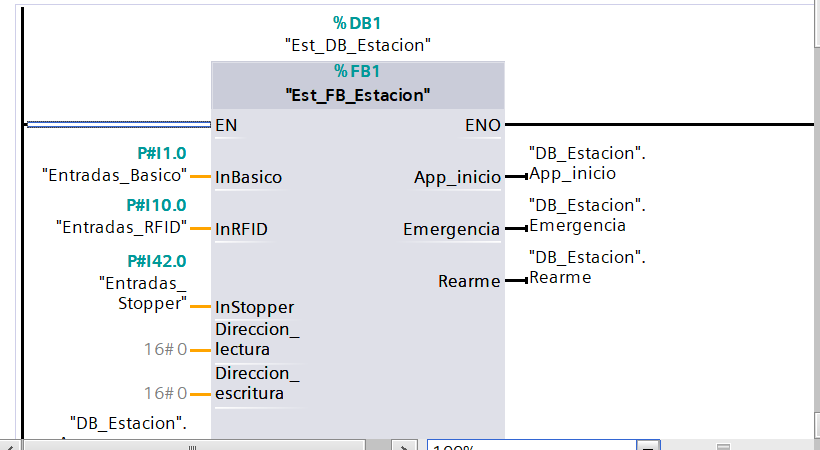
\includegraphics[width=0.92\textwidth]{capturas/main_red1.png}
\caption{La llamada a \cod{Est\_FB\_Estacion} en \cod{Main} (captura de TIA Portal). A la izquierda, las entradas; a la derecha, las salidas. Los valores \texttt{16\#0000}, \texttt{16\#00620220} y \texttt{16\#0FFFFFFF} son los de la estación Out.}
\end{figure}

\subsection{Red 1: la librería}
Llama a \cod{Est\_FB\_Estacion} con su bloque de datos de instancia (TIA lo crea) y cablea cada pin así:

\begin{center}
\footnotesize
\begin{tabularx}{\textwidth}{>{\ttfamily}p{3.5cm}>{\ttfamily}p{5.3cm}X}
\toprule
\textnormal{\textbf{Pin}} & \textnormal{\textbf{Conéctalo a}} & \textbf{Notas} \\
\midrule
InBasico & "Entradas\_Basico" & Igual en todas las estaciones. \\
InRFID & "Entradas\_RFID" & Igual en todas. \\
InStopper & "Entradas\_Stopper" & Igual en todas. \\
Direccion\_lectura & 16\#0000 & Dirección de inicio del bloque (sección~\ref{sec:calculo-mascara}). \\
Direccion\_escritura & 16\#0000 & Igual que la anterior. \\
Mascara\_lectura & \textbf{la tuya} & Capítulo~\ref{cap:mapa}. \\
Mascara\_escritura & \textbf{la tuya} & Capítulo~\ref{cap:mapa}. \\
App\_en\_reposo & "DB\_Estacion".App\_en\_reposo & Contrato. \\
App\_terminada & "DB\_Estacion".App\_terminada & Contrato. \\
App\_alarma & "DB\_Estacion".App\_alarma & Contrato. \\
App\_rearme\_requerido & "DB\_Estacion".App\_rearme\_requerido & Contrato. \\
Inhibir\_cinta & "DB\_Estacion".Inhibir\_cinta & Contrato. \\
App\_inicio (salida) & "DB\_Estacion".App\_inicio & Contrato. \\
Emergencia (salida) & "DB\_Estacion".Emergencia & Contrato. \\
Rearme (salida) & "DB\_Estacion".Rearme & Contrato. \\
OutBasico & "Salidas\_Basico" & Igual en todas. \\
OutRFID & "Salidas\_RFID" & Igual en todas. \\
Imagen\_palet & "DB\_Estacion".Imagen\_palet & La imagen del palet. \\
\bottomrule
\end{tabularx}
\end{center}

\subsection{Red 2: tu aplicación}
Llama a tu bloque \cod{FB\_App\_}\emph{tu estación} y cablea las señales del contrato a las mismas variables de \cod{DB\_Estacion}:

\begin{center}
\footnotesize
\begin{tabularx}{\textwidth}{>{\ttfamily}p{3.5cm}>{\ttfamily}p{5.3cm}X}
\toprule
\textnormal{\textbf{Pin de tu aplicación}} & \textnormal{\textbf{Conéctalo a}} & \textbf{Dirección} \\
\midrule
App\_inicio & "DB\_Estacion".App\_inicio & entrada \\
Emergencia & "DB\_Estacion".Emergencia & entrada \\
Rearme & "DB\_Estacion".Rearme & entrada \\
App\_en\_reposo & "DB\_Estacion".App\_en\_reposo & salida \\
App\_terminada & "DB\_Estacion".App\_terminada & salida \\
App\_alarma & "DB\_Estacion".App\_alarma & salida \\
App\_rearme\_requerido & "DB\_Estacion".App\_rearme\_requerido & salida \\
Inhibir\_cinta & "DB\_Estacion".Inhibir\_cinta & salida \\
Imagen\_palet & "DB\_Estacion".Imagen\_palet & entrada/salida \\
\textit{(tus señales físicas)} & \textit{tus tags} & según tu estación \\
\bottomrule
\end{tabularx}
\end{center}

\begin{consejo}
Cablea los pines de tus señales físicas \textbf{directamente a los tags de tu módulo}, por ejemplo \cod{"Entradas\_APP".Eje\_z\_arriba}. Es la manera más clara: ves de un vistazo qué sensor entra en qué pin.
\end{consejo}

\paso{Compila}
Compila todo el software. Los errores típicos de esta fase y su solución están en el capítulo~\ref{cap:problemas}.

\comprobar{0 errores. Un aviso sobre direcciones de hardware que no existen es normal si aún no has ajustado tu configuración.}

\section{Datos del RFID con un formato propio}\label{sec:rfid-propio}
Si tu código antiguo ya trabajaba con el tag a su manera, esto es lo que hay que cambiar según el caso.

\begin{description}[style=nextline,leftmargin=1.2cm]
\item[Leías el array de 28 bytes directamente (\cod{Entradas\_RFID.Tag\_datos\_leidos\_escritos[n]}).] Sustitúyelo por \cod{Imagen\_palet[n]}. El índice $n$ es el mismo (es el offset dentro del bloque). Añade el byte $n$ a \cod{Mascara\_lectura}.
\item[Usabas una palabra (un \texttt{Word} o un \texttt{Int}) en una dirección.] Es lo que hacía la práctica con CIROS. Ahora hay que partirla en dos bytes. Con el formato del grupo (big-endian), la palabra de los bytes $n$ y $n+1$ es:
\begin{lstlisting}
#valor := WORD_TO_INT(SHL(IN := BYTE_TO_WORD(#Imagen_palet[#IDX_ALTO]), N := 8)
                      OR BYTE_TO_WORD(#Imagen_palet[#IDX_BAJO]));
\end{lstlisting}
y al revés, para escribirla, con \cod{\#Imagen\_palet[\#IDX\_ALTO]} y \cod{[\#IDX\_BAJO]} cogiendo el byte alto y el bajo del valor. Los dos bytes tienen que estar en tus máscaras.
\item[Leías en otra dirección distinta de 0.] Pon esa dirección en \cod{Direccion\_lectura} y \cod{Direccion\_escritura} (las dos iguales). Los índices de la imagen son \emph{relativos al comienzo del bloque}: el byte 0 de la imagen es el primero del bloque, estés donde estés en el tag.
\item[Tu estación guardaba cosas en bytes que el mapa no contempla.] No lo hagas sin acordarlo: habla con el grupo, añade el campo al Excel (capítulo~\ref{cap:mapa}) y entonces úsalo.
\item[Necesitas más de 28 bytes.] No es posible con esta versión: el bloque es de 28 bytes. Habría que plantear una versión nueva de la librería (capítulo~\ref{cap:mantenimiento}).
\end{description}

\section{Tres ejemplos resueltos}
El apéndice~\ref{ap:listados} trae tres aplicaciones de ejemplo completas, con la parte del tag ya hecha según el Excel. Son \textbf{puntos de partida}: la parte física (nombres de sensores y actuadores) es de ejemplo y cada grupo la sustituye por la suya. Los tres compilan en TIA y se han probado en el simulador de la librería.

\begin{center}
\small
\begin{tabularx}{\textwidth}{>{\bfseries}p{2.4cm}p{3.7cm}X}
\toprule
Estación & Qué hace con el tag & Estados de la aplicación \\
\midrule
Press (\cod{FB\_App\_Press\_Ejemplo}) & Lee golpes y tiempo; escribe golpes realizados y su bit de «completada». & Reposo $\rightarrow$ bajar $\rightarrow$ mantener $\rightarrow$ subir (se repite $n$ veces) $\rightarrow$ escribir $\rightarrow$ fin. \\
BackCover (\cod{FB\_App\_BackCover\_Ejemplo}) & Marca estado de la tapa trasera (requerida, colocada, falta stock) y su bit. & Reposo $\rightarrow$ colocar (o falta stock) $\rightarrow$ fin. \\
Cámara (\cod{FB\_App\_Camara\_Ejemplo}) & Inicializa el bloque si está vacío; elige el job; escribe resultado, calidad, ImageID e intentos. & Reposo $\rightarrow$ inspeccionar $\rightarrow$ resultado $\rightarrow$ fin (con fallo posible). \\
\bottomrule
\end{tabularx}
\end{center}

\subsection{Qué comparten los tres}
Los tres siguen la misma estructura, que es la que te recomiendo para tu propia aplicación:
\begin{enumerate}
\item Las salidas se ponen a su valor seguro al principio de cada ciclo; cada estado activa las que necesite.
\item En el reposo, antes de empezar, se comprueba si la estación se pide (\emph{«estaciones a realizar»}, byte 3). Si no se pide, el palet pasa sin tocar nada. Esto lo exige el mapa del grupo: un byte 3 a 0 significa que actúan todas.
\item Solo se marca el bit de «completada» (byte 4) si de verdad se ha hecho el trabajo.
\item El estado de fin mantiene \cod{App\_terminada} hasta que \cod{App\_inicio} baja.
\item Emergencia: vuelta a reposo y actuadores apagados.
\end{enumerate}

\subsection{Cómo cablear sus señales físicas en \texttt{Main}}
Por ejemplo, la llamada de Press añade, a los nueve pines del contrato, estas señales propias:
\begin{center}
\small
\begin{tabularx}{\textwidth}{>{\ttfamily}p{4.4cm}>{\ttfamily}p{4.4cm}X}
\toprule
\textnormal{\textbf{Pin (de ejemplo)}} & \textnormal{\textbf{Tu tag}} & \textbf{Qué es} \\
\midrule
Prensa\_arriba & "Entradas\_APP".\textit{tu sensor} & Final de carrera superior. \\
Prensa\_presion\_inferior & "Entradas\_APP".\textit{tu sensor} & Presión inferior alcanzada. \\
Hay\_tapa\_trasera & "Entradas\_APP".\textit{tu sensor} & Hay tapa trasera en el palet. \\
Prensa\_bajar (salida) & "Salidas\_APP".\textit{tu actuador} & Bajar la prensa. \\
Prensa\_subir (salida) & "Salidas\_APP".\textit{tu actuador} & Subir la prensa. \\
\bottomrule
\end{tabularx}
\end{center}

\section{Casos especiales}
\begin{description}[style=nextline,leftmargin=1.2cm]
\item[Tu mecanismo estorba a la cinta.] Activa \cod{Inhibir\_cinta} mientras estorbe. Out lo hace con el eje Z: la cinta solo se mueve con Z arriba.
\item[Tu estación necesita rearmarse tras una emergencia que la deja a medias.] Activa \cod{App\_rearme\_requerido} hasta que te hayas recolocado, y mantén \cod{App\_en\_reposo} a falso. Mira cómo lo hace \cod{FB\_App\_Out} (estado 30).
\item[Quieres avisar de un problema sin parar la estación.] \cod{App\_alarma}. Si la haces parpadear en tu aplicación, la luz Q2 parpadea.
\item[Tu estación no usa cinta (por ejemplo, un puesto manual).] La librería no está pensada para eso; habla con el grupo antes de adaptarla.
\item[Quieres leer o escribir el tag más de una vez por palet.] La secuencia de la librería lee una vez y escribe una vez. Si necesitas algo distinto, es un cambio de la librería (capítulo~\ref{cap:mantenimiento}).
\item[Tu estación tiene una HMI propia.] La HMI lee las variables de tu aplicación y de \cod{DB\_Estacion}. La librería no escribe en ninguna pantalla.
\end{description}

\section{Lista final de la migración}
Cuando hayas terminado, comprueba esto (hay una copia imprimible en el apéndice~\ref{ap:checklists}):
\begin{itemize}
\item[$\square$] El proyecto compila sin errores.
\item[$\square$] Los cuatro FB y seis UDT de la librería siguen ligados a ella (no los has editado).
\item[$\square$] \cod{Main} llama primero a \cod{Est\_FB\_Estacion} y luego a tu aplicación.
\item[$\square$] Tus máscaras corresponden a tus bytes, y los bytes que escribes están también en la lectura.
\item[$\square$] Tu aplicación cumple las siete reglas del capítulo~\ref{cap:contrato}.
\item[$\square$] Has hecho las pruebas del capítulo~\ref{cap:pruebas}.
\item[$\square$] Tu código antiguo está en la carpeta \menu{Antiguo}, y la copia de seguridad guardada.
\end{itemize}
